\documentclass[../PhysicsFormulae.tex]{subfiles}
\begin{document}

\subsection{Conservation of Momentum}
Conservation of momentum is derived from Newton's 2nd Law, holding true when $\vec{F}=0$.
\[\vec{F} = \frac{d\vec{p}}{dt}=0 \rightarrow \vec{p}=constant\]
It can be easier to analyze collisions in the CM frame, where total momentum is 0. 

\subsection{Center Mass}
Center mass is defined as
\[\vec{r}_{cm} = \frac{\sum m_i \vec{r}_i}{M}\]
Taking some derivatives yields
\[\vec{v}_{cm} = \frac{\sum m_i \vec{v}_i}{M}\]
and
\[\vec{a}_{cm} = \frac{\sum m_i \vec{a}_i}{M}\]

\subsubsection{Triangular Plate}
The CM of a triangular plate follows from symmetry; it lies on the intersection of the three medians of the triangle.

\subsubsection{Hollow Hemisphere}
The CM of an empty half-sphere is given by
\[y_{cm} = \frac{R}{2}\]
where $y_{cm}$ is measured from the center of the sphere.

\subsubsection{Solid Hemisphere}
The CM of a solid half-sphere is given by 
\[y_{cm} = \frac{3R}{8}\]
where $y_{cm}$ is measured from the center of the sphere.

\subsection{Elastic Collisions}
In linear elastic collisions, the velocities in the CM frame simply reverse. In higher dimensions, the objects' velocities remain anti-parallel, but they may be redirected at an angle.\bigskip

Working in the lab frame, for initial velocities $v_1$ and $v_2$, and CM velocity 
\[v_{cm}=\frac{m_1v_1 + m_2v_2}{m_1 + m_2}\]

the final velocities (for a 1D collision) are given by
\[u_1 = 2v_{cm} - v_1\]
\[u_2 = 2v_{cm} - v_2\]
Elastic collisions in 2D should be analyzed in the following way:
\begin{itemize}
    \item Perpendicular deflections can be solved by applying the Pythagorean theorem to the momenta, with initial momentum as hypotenuse and final momenta as legs. 
    \item When the masses are identical, it is best to analyze in the CM frame. 
\end{itemize}
\begin{figure}
    \centering
    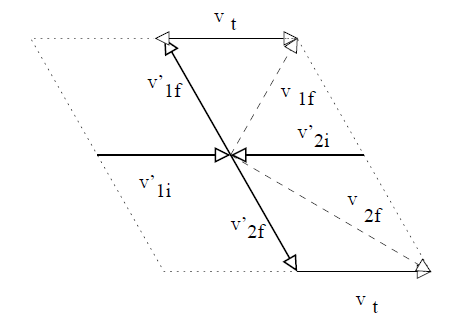
\includegraphics[width=0.5\linewidth]{images/5.identical_mass_velocity_transform.png}
    \caption{Initial and final velocities in the CM and lab frames}
    \label{fig:vdiagram1}
\end{figure}
As shown in the diagram, primed velocities denote the CM frame and unprimed ones denote the lab frame. Note that the diagonals of a rhombus (and thus the final velocities) must be at right angles. 
\subsection{Inelastic Collisions}
Perfectly inelastic collisions cause objects to stick together. 

\subsection{Variable Mass Systems}
When the mass of a system is changing, such as in rockets, apply
\[\sum F_{ext} + v_{rel}\frac{dm}{dt} = m\frac{dv}{dt}\]

In the special case $\sum F_{ext} = 0$ this becomes
\[v_2 = v_1 + v_{rel}\ln{\frac{m_2}{m_1}}\]

\end{document}